
% header %{{{1

\documentclass[tikz, border=1mm]{standalone}

\usepackage{amsmath}

\usetikzlibrary{calc,angles,quotes,intersections,shapes.geometric}

\usepackage{tkz-euclide}

% document %{{{1

% opening %{{{2

\begin{document}
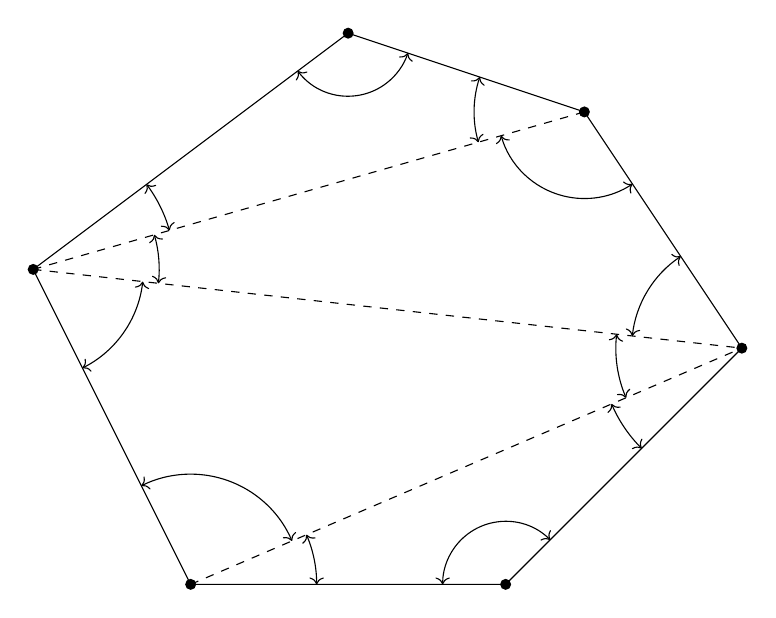
\begin{tikzpicture}[scale=1.0]

% coordinates %{{{2

	\coordinate (P1) at (0,0);
	\coordinate (P2) at (-2,4);
	\coordinate (P3) at (2,7);
	\coordinate (P4) at (5,6);
	\coordinate (P5) at (7,3);
	\coordinate (P6) at (4,0);

% polygon %{{{2

	\draw (P1) \foreach \i in {2,...,6} { -- (P\i) } -- cycle;

% triangles %{{{2

	\draw[dashed] (P2) -- (P4);
	\draw[dashed] (P2) -- (P5);
	\draw[dashed] (P1) -- (P5);

% points, dots, vertices %{{{2

	\foreach \i in {1,...,6} { \fill (P\i) circle (0.7mm); }

% angles labels %{{{2

	\pic[draw, <->, angle radius=1.6cm, angle eccentricity=1.0]
	{angle = P6--P1--P5};

	\pic[draw, <->, angle radius=1.4cm, angle eccentricity=1.0]
	{angle = P5--P1--P2};

	\pic[draw, <->, angle radius=1.4cm, angle eccentricity=1.0]
	{angle = P1--P2--P5};

	\pic[draw, <->, angle radius=1.6cm, angle eccentricity=1.0]
	{angle = P5--P2--P4};

	\pic[draw, <->, angle radius=1.8cm, angle eccentricity=1.0]
	{angle = P4--P2--P3};

	\pic[draw, <->, angle radius=0.8cm, angle eccentricity=1.0]
	{angle = P2--P3--P4};

	\pic[draw, <->, angle radius=1.4cm, angle eccentricity=1.0]
	{angle = P3--P4--P2};

	\pic[draw, <->, angle radius=1.1cm, angle eccentricity=1.0]
	{angle = P2--P4--P5};

	\pic[draw, <->, angle radius=1.4cm, angle eccentricity=1.0]
	{angle = P4--P5--P2};

	\pic[draw, <->, angle radius=1.6cm, angle eccentricity=1.0]
	{angle = P2--P5--P1};

	\pic[draw, <->, angle radius=1.8cm, angle eccentricity=1.0]
	{angle = P1--P5--P6};

	\pic[draw, <->, angle radius=0.8cm, angle eccentricity=1.0]
	{angle = P5--P6--P1};

% closing %{{{2

\end{tikzpicture}
\end{document}
